% Fig 2.10 -- the increment of the cdf over a short interval [x, x+Delta x]
% No manuscript tikzpicture exists for this one; it is drawn for the web so
% that it shares curve, x range, scale and axis length with Figs 2.8, 2.11
% and 2.12 (specs Fig A04, A06, A07 of CH2_FIGURE_SPECS.md).
% Density: true N(3,1), f(t) = 0.3989423 e^{-(t-3)^2/2}, integrates to 1.
% Drawing scale x=1.15cm, y=8.74cm; peak f(3) = 0.3989423 -> 3.4868cm.
% Shaded region: [3.3, 4.0], i.e. x = 3.3 and Delta x = 0.7.
\documentclass[tikz,border=2pt]{standalone}
\usepackage{amsmath}
\usepackage{amssymb}
\usepackage{xcolor}
\usetikzlibrary{arrows.meta}
\newcommand{\sssig}{\scriptscriptstyle}

\definecolor{journalink}{HTML}{1F1C18}
\definecolor{journalmuted}{HTML}{8A7F72}
\definecolor{journalaccent}{HTML}{9C2D2D}

\begin{document}
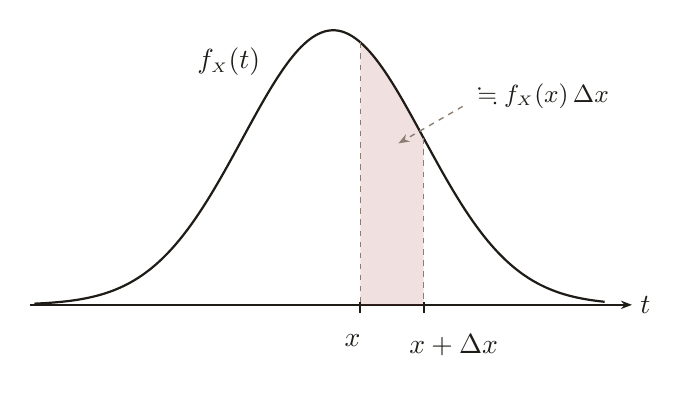
\begin{tikzpicture}[
  x=1.15cm,
  y=8.74cm,
  every node/.style={font=\normalsize, journalink},
  axis/.style={journalink, line width=0.8pt, -{Stealth[length=4pt]}},
  tick/.style={journalink, line width=0.8pt},
  curve/.style={journalink, line width=0.8pt},
  guide/.style={journalmuted, line width=0.5pt, dash pattern=on 2pt off 2pt},
  region/.style={journalaccent, fill opacity=0.15},
  pointer/.style={journalmuted, line width=0.5pt,
                  dash pattern=on 2pt off 2pt, -{Stealth[length=4pt]}}
]
  % ---- common bounding box, identical in all four figures of this group ----
  \path (-0.43cm,-0.78cm) rectangle (7.58cm,3.52cm);

  % ---- x axis ----
  \draw[axis] (-0.35,0) -- (6.3,0);

  % ---- shaded strip over [3.3, 4.0] ----
  \fill[region]
    (3.3,0) -- (4,0) -- (4,0.2419707)
    -- plot[domain=4:3.3, samples=200, smooth]
       (\x,{0.3989423*exp(-(\x-3)*(\x-3)/2)})
    -- cycle;

  % ---- density curve: N(3,1) ----
  \draw[curve] plot[domain=-0.3:6, samples=200, smooth]
    (\x,{0.3989423*exp(-(\x-3)*(\x-3)/2)});

  % ---- the two boundaries of the strip ----
  \draw[guide] (3.3,0.3813878) -- (3.3,0);
  \draw[guide] (4,0.2419707) -- (4,0);
  \draw[tick] ([yshift=0.035cm]3.3,0) -- ([yshift=-0.106cm]3.3,0);
  \draw[tick] ([yshift=0.035cm]4,0) -- ([yshift=-0.106cm]4,0);
  % the two labels are nudged apart (0.10cm left, 0.38cm right) so that their
  % ink clears by 0.62cm, above the 0.6cm required by spec 1.3
  \node[anchor=north, xshift=-0.10cm] at ([yshift=-0.25cm]3.3,0) {$x$};
  \node[anchor=north, xshift=0.38cm] at ([yshift=-0.25cm]4,0) {$x+\Delta x$};

  % ---- callout for the shaded strip ----
  \draw[pointer] (4.43,0.2883295) -- (3.72,0.2345538);
  \node[anchor=east, inner sep=0pt] at ([yshift=2.65cm]6.05,0)
    {\small $\fallingdotseq f_{\sssig X}(x)\,\Delta x$};

  % ---- labels ----
  \node[anchor=south east, inner sep=0pt] at ([yshift=0.38cm]2.2,0.2896916)
    {$f_{\sssig X}(t)$};
  \node[anchor=west, inner sep=2.8pt] at (6.3,0) {$t$};
\end{tikzpicture}
\end{document}
